\begin{enumerate}[(a)]
\item \textbf{\underline{C.I., Wald test and Likelihood Ratio test: MAC Dataset.}} After importing the data into \verb|R|, we can see few lines of the data by typing:
\begin{footnotesize}
\begin{verbatim}
> #####################################################
> ### LAB 5: More on Cox Proportional Hazards Model ###
> #####################################################
> 
> # MAC dataset, here we're interested in time to MAC disease
> # NOT time to death
> mac = read.csv("C:/Applied_Survival_Analysis_Jan2016/lab5/data/mac.csv")
> 
> # See some lines of the data
> mac[1:10,c("patid","macstat","mactime","karnof","rif","clari","cd4")]
   patid macstat mactime karnof rif clari cd4
1      1       1     560     90   1     0   8
2      2       0     651     90   1     0  30
3      3       0      26    100   1     0  80
4      4       0     622     80   0     1  58
5      5       0     643     90   0     1  59
6      6       0     171     90   0     1  18
7      7       1     174     90   0     0  20
8      8       1     449     90   1     0  30
9      9       1     377     80   0     0  30
10    10       0      58     60   1     0  20
\end{verbatim}
\end{footnotesize}
In this lab, we're interested in time to MAC disease (variable \emph{mactime}). The corresponding failure indicator is the variable \emph{macstat}. To see the number of events of interest, we can use the \verb|table| function, which returns a frequency table. Also you can get some descriptive statistics regarding the time variable using the function \verb|summary|. Please, see ?\verb|table| and ?\verb|summary| if you want more details.
\begin{footnotesize}
\begin{verbatim}
> # Number of events
> table(mac$macstat)

   0    1 
1056  121 
> summary(mac$mactime)
   Min. 1st Qu.  Median    Mean 3rd Qu.    Max. 
    0.0   171.0   447.0   415.9   641.0   827.0 
\end{verbatim}
\end{footnotesize}
We'd better exclude the patients with zero event times, although such cases are always excluded by the program when a survival model is fitted.
\begin{footnotesize}
\begin{verbatim}
> # Delete 26 patients with zero time
> table(mac$mactime==0)

FALSE  TRUE 
 1151    26 
> mac = mac[mac$mactime!=0,]
\end{verbatim}
\end{footnotesize}
\begin{enumerate}[(i)]
\item Now, we're going to fit a Cox PH model including the clarithromycin and rifabutin effects along with the effects of the Karnofsky score. 
\begin{footnotesize}
\begin{verbatim}
> # (a)-(i): Time to MAC disease in relation
> # to karnofsky score and treatment group
> library(survival)
> fit.mac1 = coxph( Surv(mactime,macstat) ~ karnof + rif + clari,data = mac)
> summary(fit.mac1)
Call:
coxph(formula = Surv(mactime, macstat) ~ karnof + rif + clari, 
    data = mac)

  n= 1151, number of events= 121 

           coef exp(coef) se(coef)      z Pr(>|z|)    
karnof -0.04485   0.95614  0.01064 -4.217 2.48e-05 ***
rif     0.87197   2.39161  0.23694  3.680 0.000233 ***
clari   0.27557   1.31728  0.25801  1.068 0.285509    
---
Signif. codes:  0 ‘***’ 0.001 ‘**’ 0.01 ‘*’ 0.05 ‘.’ 0.1 ‘ ’ 1

       exp(coef) exp(-coef) lower .95 upper .95
karnof    0.9561     1.0459    0.9364    0.9763
rif       2.3916     0.4181    1.5032    3.8051
clari     1.3173     0.7591    0.7944    2.1842

Concordance= 0.649  (se = 0.028 )
Rsquare= 0.027   (max possible= 0.738 )
Likelihood ratio test= 32.02  on 3 df,   p=5.193e-07
Wald test            = 32.29  on 3 df,   p=4.548e-07
Score (logrank) test = 33.16  on 3 df,   p=2.977e-07
\end{verbatim}
\end{footnotesize}
Please, note that since we have only included the rifabutin
and clarithromycin effects in the model, the combination therapy is the
“reference” group. The hazard ratio of the Karnofsky score status is 
$HR = \exp(-0.0448)=0.956$. 
After adjusting for the effect of treatment, the hazard of MAC disease is 
approximately 4\% less for each unit increase in the Karnofsky score.
\item When constructing a confidence interval for a hazard ratio, it's better to first construct a confidence interval for the $\log(HR)$, and then back-transform (exponentiate) the endpoints to the hazard ratio scale. In \verb|R|, the \verb|confint| function gives the CIs of the $\log(HR)$, thus
\begin{footnotesize}
\begin{verbatim}
> # (a)-(ii): Contruncting 95% CIs for the hazard ratios
> # First calculate CI's for log(HR) and 
> # then back-transform to the HR scale
> exp(confint(fit.mac1))
           2.5 %    97.5 %
karnof 0.9364180 0.9762838
rif    1.5031710 3.8051475
clari  0.7944283 2.1842323
\end{verbatim}
\end{footnotesize}
Alternatively, we can construct the CIs by taking advantage of the \verb|vcov| function, which gives the estimated covariance matrix of parameter estimates (command \verb|mat li e(V)| in \verb|STATA|). Note that the standard errors of parameter estimates are the square roots of the diagonal elements of this matrix.
In \verb|R|, the function \verb|diag| extracts the diagonal elements of a matrix, and the \verb|coef| function extracts parameter estimates from objects  returned by modelling functions (see ?\verb|coef| and ?\verb|diag| for more details)   
\begin{footnotesize}
\begin{verbatim}
> # or,
> exp( cbind( coef(fit.mac1)-qnorm(0.975)*sqrt(diag(vcov(fit.mac1))),
+        coef(fit.mac1),
+        coef(fit.mac1)+qnorm(0.975)*sqrt(diag(vcov(fit.mac1))) ))
            [,1]      [,2]      [,3]
karnof 0.9364180 0.9561432 0.9762838
rif    1.5031710 2.3916077 3.8051475
clari  0.7944283 1.3172760 2.1842323
\end{verbatim}
\end{footnotesize}
Thus, the 95\%CI for the hazard ratio of the Karnofsky score status is $[0.936,0.976]$. This 
implies 2\% to 6\% decrease in hazard of MAC disease for each unit increase in the 
Karnofsky score after adjusting for the treatment effect
\item The null and 
alternative hypothesis are
\begin{align}
\begin{cases}
H0: & \beta_{karnof} = 0 \\
H1: & \beta_{karnof} \neq 0
\end{cases}\nonumber
\end{align}
The Wald test is constructed by dividing the model coefficient by its standard error, and squaring the result
\begin{footnotesize}
\begin{verbatim}
> # (a)-(iii): Wald test for the karnofsky score
> z.tests = coef(fit.mac1)/sqrt(diag(vcov(fit.mac1)))
> chi2 = z.tests^2
> chi2[1]
  karnof 
17.78044
\end{verbatim}
\end{footnotesize}
\item Next we want to add the effect of CD4, so we need to fit the following model:
\begin{footnotesize}
\begin{verbatim}
> # a-(iv): Add CD4 cell count in the model
> fit.mac2 = coxph( Surv(mactime,macstat) ~ karnof + rif + clari + cd4,data = mac)
> summary(fit.mac2)
Call:
coxph(formula = Surv(mactime, macstat) ~ karnof + rif + clari + 
    cd4, data = mac)

  n= 1151, number of events= 121 

            coef exp(coef)  se(coef)      z Pr(>|z|)    
karnof -0.036874  0.963798  0.010665 -3.457 0.000546 ***
rif     0.879749  2.410294  0.237092  3.711 0.000207 ***
clari   0.252345  1.287041  0.258337  0.977 0.328664    
cd4    -0.018360  0.981807  0.003684 -4.984 6.23e-07 ***
---
Signif. codes:  0 ‘***’ 0.001 ‘**’ 0.01 ‘*’ 0.05 ‘.’ 0.1 ‘ ’ 1

       exp(coef) exp(-coef) lower .95 upper .95
karnof    0.9638     1.0376    0.9439    0.9842
rif       2.4103     0.4149    1.5145    3.8360
clari     1.2870     0.7770    0.7757    2.1354
cd4       0.9818     1.0185    0.9747    0.9889

Concordance= 0.716  (se = 0.028 )
Rsquare= 0.054   (max possible= 0.738 )
Likelihood ratio test= 63.77  on 4 df,   p=4.682e-13
Wald test            = 55.59  on 4 df,   p=2.449e-11
Score (logrank) test = 56.22  on 4 df,   p=1.806e-11
\end{verbatim}
\end{footnotesize}
To get the likelihood ratio test that evaluates the significance of CD4, we need to fit a model without CD4 and one with CD4. Recall that these models have been saved in objects called \verb|fit.mac1| and \verb|fit.mac2|, respectively. Then, by using the \verb|anova| function you can easily get the LR test
\begin{footnotesize}
\begin{verbatim}
> # LR test comparing the model with and without CD4
> anova(fit.mac1,fit.mac2)
Analysis of Deviance Table
 Cox model: response is  Surv(mactime, macstat)
 Model 1: ~ karnof + rif + clari
 Model 2: ~ karnof + rif + clari + cd4
   loglik Chisq Df P(>|Chi|)    
1 -754.49                       
2 -738.62 31.75  1 1.754e-08 ***
---
Signif. codes:  0 ‘***’ 0.001 ‘**’ 0.01 ‘*’ 0.05 ‘.’ 0.1 ‘ ’ 1
> 
> # or,
> -2*(fit.mac1$loglik - fit.mac2$loglik)[2]
[1] 31.74965
\end{verbatim}
\end{footnotesize}
Please also note that you can get the log partial likelihood from a \verb|coxph| object by typing \verb|fit.mac1$loglik|. This gives us a vector of size 2, where the first element is the loglikelihood of the null model whereas the second element is the loglikelihood of the fitted model.

The result of the above LR test implies that the addition of CD4 contributes significantly in 
predicting MAC disease.
\item To evaluate the overall significance of treatment, we can construct a multivariate Wald test (see the GLM notes or page 4 of lecture 5).
\begin{footnotesize}
\begin{verbatim}
> # (a)-(v): Test for an overall treatment effect using a (multivariate) Wald test
> # after taking into account the Karnofsky score and CD4 count
> fit.mac2 = coxph( Surv(mactime,macstat) ~ karnof + rif + clari + cd4,data = mac)
> coef(fit.mac2)
     karnof         rif       clari         cd4 
-0.03687351  0.87974888  0.25234548 -0.01836011 
> 
> # Please, have a look at the GLM notes
> # We are contructing a chi-square test with 2 degrees of freedon
> chi2 = t(coef(fit.mac2)[2:3]) %*% solve(vcov(fit.mac2)[2:3,2:3]) %*% coef(fit.mac2)[2:3]
> chi2
         [,1]
[1,] 17.00252
> 
> # p-value
> 1-pchisq(chi2,df=2)
             [,1]
[1,] 0.0002032125
\end{verbatim}
\end{footnotesize}
Please, make sure you wrote \verb|solve(vcov(fit.mac2)[2:3,2:3])| \\
and \textbf{not} \verb|solve(vcov(fit.mac2))[2:3,2:3]|. Results from the latter are wrong!

Treatment type seems to have a significant effect on time to MAC disease after adjusting for the Karnofsky score and CD4 levels. 

These is also an easier way to get the desired test using the function \verb|linearHypothesis| in \verb|car| library.
\begin{spacing}{1.2}
\begin{footnotesize}
\begin{verbatim}
> # or more easily
> library(car)
Warning message:
package ‘car’ was built under R version 3.1.3 
> linearHypothesis(fit.mac2,c("rif","clari"))
Linear hypothesis test

Hypothesis:
rif = 0
clari = 0

Model 1: restricted model
Model 2: Surv(mactime, macstat) ~ karnof + rif + clari + cd4

  Res.Df Df  Chisq Pr(>Chisq)    
1   1149                         
2   1147  2 17.003  0.0002032 ***
---
Signif. codes:  0 ‘***’ 0.001 ‘**’ 0.01 ‘*’ 0.05 ‘.’ 0.1 ‘ ’ 1
\end{verbatim}
\end{footnotesize}
\end{spacing} 
\item We would like to test whether there is a difference between the rifabutin and clarithromycin treatment arms. There are several ways to perform such a test, but we are going to focus on a quick way to get it, by reparameterizing
the model. If
\begin{align}
\lambda(t) = \lambda_{0}(t)\exp\left\{\beta_{1}\text{rif}+\beta_{2}\text{clari}\right\},\nonumber 
\end{align}      
we are interested in testing $\beta_{1}=\beta_{2}$. However, this is equivalent to testing $\beta_{1}-\beta_{2} = \alpha = 0$. So,
\begin{align}
\lambda(t) &= \lambda_{0}(t)\exp\left\{(\beta_{2}+\alpha)\text{rif}+\beta_{2}\text{clari}\right\} \nonumber \\
\lambda(t) &= \lambda_{0}(t)\exp\left\{\alpha \text{rif}+\beta_{2}[\text{rif}+\text{clari}]\right\} \nonumber
\end{align}
Thus, to get the desired test we can equivalently test $\alpha=0$. Using \verb|R| code
\begin{footnotesize}
\begin{verbatim}
> # a-(vi): To test whether there is a DIFFERENCE between the 
> # rif and clari treatment arms, 
> # see the coefficient of rif 
> fit.mac3 = coxph( Surv(mactime,macstat) ~ karnof + rif + I(rif + clari) + cd4,data = mac)
> summary(fit.mac3)
Call:
coxph(formula = Surv(mactime, macstat) ~ karnof + rif + I(rif + 
    clari) + cd4, data = mac)

  n= 1151, number of events= 121 

                    coef exp(coef)  se(coef)      z Pr(>|z|)    
karnof         -0.036874  0.963798  0.010665 -3.457 0.000546 ***
rif             0.627403  1.872742  0.211970  2.960 0.003078 ** 
I(rif + clari)  0.252345  1.287041  0.258337  0.977 0.328664    
cd4            -0.018360  0.981807  0.003684 -4.984 6.23e-07 ***
---
Signif. codes:  0 ‘***’ 0.001 ‘**’ 0.01 ‘*’ 0.05 ‘.’ 0.1 ‘ ’ 1

               exp(coef) exp(-coef) lower .95 upper .95
karnof            0.9638      1.038    0.9439    0.9842
rif               1.8727      0.534    1.2361    2.8373
I(rif + clari)    1.2870      0.777    0.7757    2.1354
cd4               0.9818      1.019    0.9747    0.9889

Concordance= 0.716  (se = 0.028 )
Rsquare= 0.054   (max possible= 0.738 )
Likelihood ratio test= 63.77  on 4 df,   p=4.682e-13
Wald test            = 55.59  on 4 df,   p=2.449e-11
Score (logrank) test = 56.22  on 4 df,   p=1.806e-11
\end{verbatim}
\end{footnotesize}
The \verb|I| function was used to create a new variable that contains the sum of the variables \emph{rif} and \emph{clari}. Also, keep in mind that this new variable has not been saved in the data frame \emph{mac}. 
Note that given the way we have parametrised the model, we're interested in the coefficient of \emph{rif}, which yields a p-value of  0.0031. Thus, there is a significant difference between the rifabutin and clarithromycin arms after taking into account the karnofsky score and the CD4 levels. Alternatively,
\begin{spacing}{1.2}
\begin{footnotesize}
\begin{verbatim}
> # or,
> linearHypothesis(fit.mac2,c("rif = clari"))
Linear hypothesis test

Hypothesis:
rif - clari = 0

Model 1: restricted model
Model 2: Surv(mactime, macstat) ~ karnof + rif + clari + cd4

  Res.Df Df  Chisq Pr(>Chisq)   
1   1148                        
2   1147  1 8.7608   0.003078 **
---
Signif. codes:  0 ‘***’ 0.001 ‘**’ 0.01 ‘*’ 0.05 ‘.’ 0.1 ‘ ’ 1
\end{verbatim}
\end{footnotesize}
\end{spacing}
\end{enumerate}
\item \textbf{\underline{Survival Function and Predicted Medians: Nursing Home Data.}} We consider again the dataset \emph{nurshome.csv}.
\begin{footnotesize}
\begin{verbatim}
> ##################################################################
> ### Survival Function and Predicted Medians: Nursing Home Data ###
> ##################################################################
> nurshome = read.csv("C:/Applied_Survival_Analysis_Jan2016/lab5/data/nurshome.csv")
> nurshome[1:4,]
  los age rx gender married health fail
1 665  83  1      0       0      4    1
2 697  80  0      0       0      3    0
3   7  92  1      0       0      4    1
4 217  69  0      0       0      3    1
\end{verbatim}
\end{footnotesize}
To produce a two way frequency table, you can use the \verb|table| function:
\begin{footnotesize}
\begin{verbatim}
> # Two-way frequency table
> tab = table(nurshome$married,nurshome$health)
> tab
   
      2   3   4   5
  0 299 468 417 135
  1  42 106  91  33
\end{verbatim}
\end{footnotesize}
If you would also like to add the percentages (with respect to row or column), you can use the \verb|prop.table| function
\begin{footnotesize}
\begin{verbatim}
> # To see the percentages (by rows and by col)
> prop.table(tab,1)
   
            2         3         4         5
  0 0.2266869 0.3548143 0.3161486 0.1023503
  1 0.1544118 0.3897059 0.3345588 0.1213235
> prop.table(tab,2)
   
            2         3         4         5
  0 0.8768328 0.8153310 0.8208661 0.8035714
  1 0.1231672 0.1846690 0.1791339 0.1964286
\end{verbatim}
\end{footnotesize}
\begin{enumerate}
\item First, we fit a Cox PH model focusing on the effects of marital status and health status.
\begin{footnotesize}
\begin{verbatim}
> # b-(i) : Cox PH model
> library(survival)
Loading required package: splines
> fit.cox = coxph( Surv(los,fail) ~ married + health, data = nurshome)
> summary(fit.cox)
Call:
coxph(formula = Surv(los, fail) ~ married + health, data = nurshome)

  n= 1591, number of events= 1269 

           coef exp(coef) se(coef)     z Pr(>|z|)    
married 0.29773   1.34679  0.07219 4.124 3.72e-05 ***
health  0.16607   1.18066  0.03125 5.315 1.07e-07 ***
---
Signif. codes:  0 ‘***’ 0.001 ‘**’ 0.01 ‘*’ 0.05 ‘.’ 0.1 ‘ ’ 1

        exp(coef) exp(-coef) lower .95 upper .95
married     1.347     0.7425     1.169     1.551
health      1.181     0.8470     1.111     1.255

Concordance= 0.558  (se = 0.009 )
Rsquare= 0.028   (max possible= 1 )
Likelihood ratio test= 45.5  on 2 df,   p=1.318e-10
Wald test            = 46.72  on 2 df,   p=7.164e-11
Score (logrank) test = 46.97  on 2 df,   p=6.317e-11
\end{verbatim}
\end{footnotesize}
\item We create a variable containing the groups of interest.
\begin{footnotesize}
\begin{verbatim}
> # b-(ii): Calculation of median by a KM approach
> # First, create the grouping factor
> nurshome$group = c(1*(nurshome$mar==0 & nurshome$health==2) +
+                    2*(nurshome$mar==0 & nurshome$health==5) +
+                    3*(nurshome$mar==1 & nurshome$health==2) +
+                    4*(nurshome$mar==1 & nurshome$health==5))
> 
> # We're not interested in the category of group = 0
> table(nurshome$group)

   0    1    2    3    4 
1082  299  135   42   33 
\end{verbatim}
\end{footnotesize}
But, since we're not interested in the category of \verb|group=0|, we can create a new data frame that will contain the groups of interest only
\begin{footnotesize}
\begin{verbatim}
> # We can create a new data frame excluding group = 0
> # Of course, several other options are available to deal with issue ...
> nurshome2 = nurshome[nurshome$group!=0,]
\end{verbatim}
\end{footnotesize}
To get the predicted medians using a KM approach, type the following
\begin{footnotesize}
\begin{verbatim}
> # Specify the order of the values and also label the values
> nurshome2$group = factor(nurshome2$group,levels = 1:4,labels = c("Single, healthy",
+                                                                  "Single, unhealthy",
+                                                                  "Married, healthy",
+                                                                  "Married, unhealthy"))
> 
> fit.KM = survfit( Surv(los,fail) ~ group,data = nurshome2)
> fit.KM
Call: survfit(formula = Surv(los, fail) ~ group, data = nurshome2)

                         records n.max n.start events median 0.95LCL 0.95UCL
group=Single, healthy        299   299     299    227    151     126     199
group=Single, unhealthy      135   135     135    121     62      44      81
group=Married, healthy        42    42      42     35    104      64     195
group=Married, unhealthy      33    33      33     30     23      17      68
\end{verbatim}
\end{footnotesize}
\item Alternatively, we can calculate the median times of interest after taking advantage of the Cox model we fitted in (i). However, the validity of this approach relies on the assumption of proportional hazards!

The whole idea is based on the estimation of the baseline survival function, since by using the formula, $S(t|\mathbf{z}_{i})=S_{0}(t)^{e^{\mathbf{z}_{i}^{T}\boldsymbol{\beta}}}$, we can easily estimate the survival function of any covariate pattern. Fortunately, using the \verb|survfit| function, this can be done almost directly as it involves very little programming.

When the \verb|survfit| function takes an \verb|coxph| object as an argument, it produces survival curves for each covariate pattern specified in the option \verb|newdata|. \verb|newdata| requires a data frame with the same variable names as those that appear in the \verb|coxph| formula. Then, a survival curve is produced for each row of this data frame. 
\begin{footnotesize}
\begin{verbatim}
> # b-(iii) We calculate the medians assuming proportional hazards
> newdata = data.frame(married = c(0,0,1,1),health = c(2,5,2,5))
> surv.cox = survfit(fit.cox, newdata = newdata)
> surv.cox
Call: survfit(formula = fit.cox, newdata = newdata)

  records n.max n.start events median 0.95LCL 0.95UCL
1    1591  1591    1591   1269    187     155     227
2    1591  1591    1591   1269     80      65      97
3    1591  1591    1591   1269    110      86     149
4    1591  1591    1591   1269     48      39      66
\end{verbatim}
\end{footnotesize}
\begin{table}[ht]
\caption{Median length of stay assuming proportional hazards.}
% title of Table
\centering
% used for centering table
\begin{tabular}{l c}
% centered columns (4 columns)
\hline
 Group & Predicted median  \\ \hline
 1 Single, healthy & 187 \\
 2 Single, unhealthy & 80 \\
 3 Married, healthy & 110 \\
 4 Married, unhealthy & 48 \\
\hline
\end{tabular}
\label{table:1}
\end{table}
Three options are available for estimating the baseline survival function (which is required internally): (1) The \emph{Breslow} method, (2) The \emph{Efron} method, and (3) The \emph{Kalbfleisch-Prentice} method. The default is to match with the tie handling method used in the Cox model, i.e.,
\begin{itemize}
\item \verb|ties='breslow'| in \verb|coxph| $\Rightarrow$ the \emph{Breslow} estimate for $\hat{S}_{0}(t)$
\item \verb|ties='efron'| in \verb|coxph| $\Rightarrow$ the \emph{Efron} estimate for $\hat{S}_{0}(t)$
\item \verb|ties='exact'| in \verb|coxph| $\Rightarrow$ the \emph{Kalbfleisch-Prentice} estimate for $\hat{S}_{0}(t)$
\end{itemize}
Anyway, you don't have to worry much about the method used for obtaining $\hat{S}_{0}(t)$, as the above-mentioned methods are incredibly close! However, you're strongly advised to examine ?\verb|survfit.coxph| in depth.

To get a visual picture of the survival curves predicted by \verb|survfit|, you can use the \verb|plot| function. However, you have to keep in mind that such curves are not raw KM probabilities, they are \textbf{fitted} curves that are subject to the proportional hazards assumption!
\begin{footnotesize}
\begin{verbatim}
> setwd("C:/Applied_Survival_Analysis_Jan2016/lab5/graphs")
> 
> pdf("nurshSurvEst.pdf",height = 6,width = 6)
> plot(surv.cox,mark.time = F,xlab = "Length of Stay of Resident (days)",
+      ylab = "Survival probability",lty = 1:4,
+      col = c("blue","red","green","orange"))
> legend("topright",lty = 1:4,col = c("blue","red","green","orange"),bty = "n",
+        legend = c("Single, healthy","Single, unhealthy","Married, healthy",
+                   "Married, unhealthy"))
\end{verbatim}
\end{footnotesize}
\begin{figure}[htbp]
	\centering
		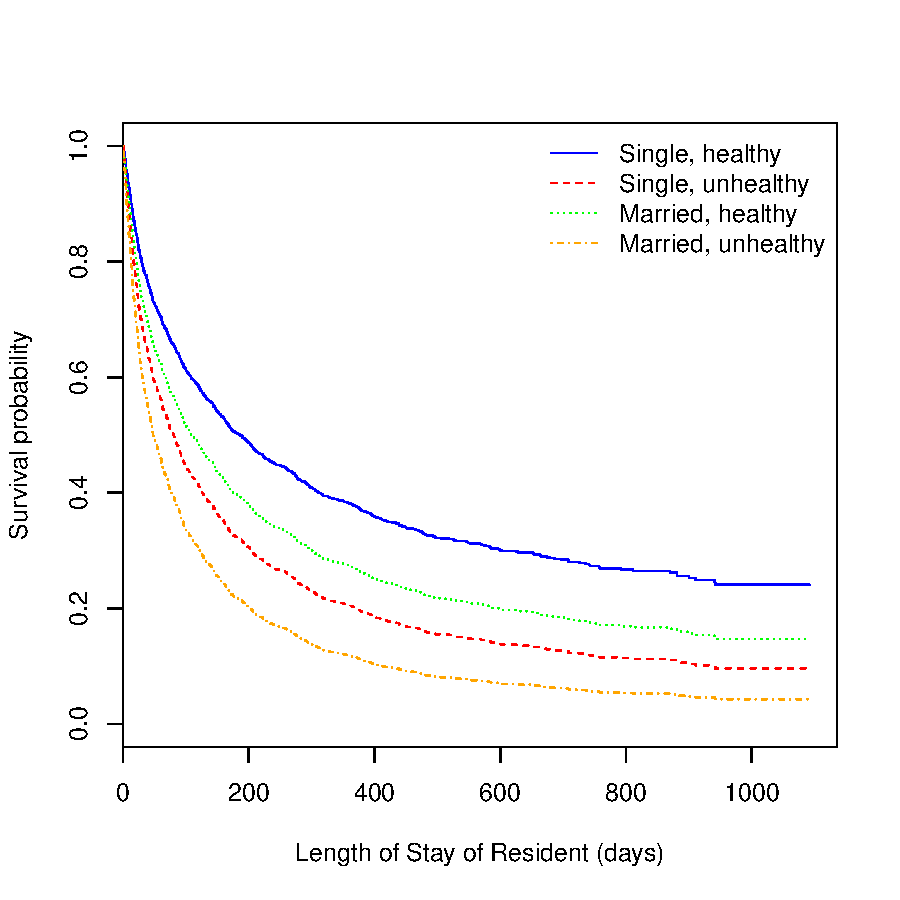
\includegraphics[scale=0.9]{nurshSurvEst.pdf}
		%\rule{35em}{0.5pt}
	\caption{Predicted survival curves for the Nursing Home Data.}
	\label{figure2}
\end{figure}
The subgroup of healthy single persons seems to have the longest length of stay. 
\newpage
\item \textbf{Optional:} The formula of the \emph{Breslow} estimator of baseline cumulative hazard is
\begin{align}
\hat{\Lambda}_{0}(t) = \sum_{j:\tau_{j}<t}\left[\dfrac{\delta_{j}}{\sum_{k\in \mathcal{R}(\tau_{j})}\exp\left\{\beta_{1}Z_{k1}+\beta_{2}Z_{k2}+\ldots+\beta_{p}Z_{kp}\right\}}
\right]. \nonumber
\end{align}
But since we're evaluating at $t^+$, we have to make the following adjustment
\begin{align}
\hat{\Lambda}_{0}(t^+) = \sum_{j:\tau_{j}\leq t}\left[\dfrac{\delta_{j}}{\sum_{k\in \mathcal{R}(\tau_{j})}\exp\left\{\beta_{1}Z_{k1}+\beta_{2}Z_{k2}+\ldots+\beta_{p}Z_{kp}\right\}}
\right]. \label{breslow}
\end{align}
We now give the \verb|R| code required to compute \eqref{breslow}. Please, don't forget to use the option \verb|type = "aalen"| to tell \verb|R| to use the \emph{Breslow} estimator of baseline cumulative hazard.
\begin{spacing}{1.1}
\begin{footnotesize}
\begin{verbatim}
> # b-(iv) Breslow estimate of baseline cumulative hazard
> # Design matrix of covariates (Don't include an intercept!)
> x = cbind(nurshome$married,nurshome$health)
> beta.hat = coef(fit.cox)
> 
> brescHaz = function(surv,fail,x,beta)
+ {
+   # Sort data with respect to time
+   data = cbind(surv,fail,x)
+   data = data[order(surv),]
+   
+   time = data[,1]
+   delta = data[,2]
+   x = data[,3:ncol(data)]
+   
+   # Distinct event times
+   times.uni = unique(time[delta==1])
+   K = length(times.uni)
+   n = length(time)
+   
+   # Number of failures for each event time
+   dj = table(time[delta==1])
+   
+   # Find where each risk set starts
+   ind = match(times.uni,time)
+   
+   # Linear predictor,
+   # %*% denotes matrix multiplication
+   Xbeta = c(x %*% beta)
+   eXbeta = exp(Xbeta)
+   
+   # Breslow estimate of baseline cumulative hazard
+   BrcumHaz = rep(NA,K)
+   
+   for (i in 1:K)
+   {
+     BrcumHaz[i] = dj[i]/sum(eXbeta[ind[i]:n])
+   }
+   BrcumHaz = cumsum(BrcumHaz)
+   
+   out = data.frame(time = times.uni, surv0 = exp(-BrcumHaz))
+   return(out)
+ }
> 
> # Our estimation
> fit = brescHaz(nurshome$los,nurshome$fail,x,beta.hat)
> 
> # Using survfit
> fit2 = survfit(fit.cox,newdata = data.frame(married = 0,health = 0),type = "aalen")
> 
> # Compare
> fit[1:10,]
   time     surv0
1     1 0.9925974
2     2 0.9868363
3     3 0.9837613
4     4 0.9779400
5     5 0.9703759
6     6 0.9651742
7     7 0.9589051
8     8 0.9539922
9     9 0.9483549
10   10 0.9441026
> cbind(summary(fit2)$time,summary(fit2)$surv)[1:10,]
      [,1]      [,2]
 [1,]    1 0.9925974
 [2,]    2 0.9868363
 [3,]    3 0.9837613
 [4,]    4 0.9779400
 [5,]    5 0.9703759
 [6,]    6 0.9651742
 [7,]    7 0.9589051
 [8,]    8 0.9539922
 [9,]    9 0.9483549
[10,]   10 0.9441026
> 
> sum(fit$surv - summary(fit2)$surv)
[1] -7.049916e-15
\end{verbatim}
\end{footnotesize}
\end{spacing}
which are exactly the same. 
\end{enumerate}
\end{enumerate}






















